\documentclass[a4paper,AutoFakeBold,AutoFakeSlant]{ctexart}
\usepackage[a4paper,left=3cm,right=3cm,top=2.5cm,bottom=2.5cm]{geometry}
\usepackage{graphicx}
\usepackage{pythonhighlight}
\usepackage[mathscr]{eucal}
\usepackage{mathrsfs}
\usepackage{booktabs}
\usepackage{capt-of} 
\usepackage{hyperref} 
\usepackage{abstract}
\usepackage{amsmath}
\usepackage{listings}
\usepackage{color}
\usepackage{caption}
\usepackage{subfigure}
\usepackage{enumerate}
\usepackage{amsfonts} 
% \usepackage{CJK,CJKnumb}
\usepackage{float}
\usepackage{gbt7714}
\usepackage{framed}


\newcommand{\song}{\CJKfamily{song}}    % 宋体   (Windows自带simsun.ttf)
\newcommand{\fs}{\CJKfamily{fs}}        % 仿宋体 (Windows自带simfs.ttf)
\newcommand{\kai}{\CJKfamily{kai}}      % 楷体   (Windows自带simkai.ttf)
\newcommand{\hei}{\CJKfamily{hei}}      % 黑体   (Windows自带simhei.ttf)
\newcommand{\li}{\CJKfamily{li}}        % 隶书   (Windows自带simli.ttf) 
\newcommand{\ssong}{\CJKfamily{STSong}}

\xeCJKsetup{SlantFactor = 0.3}
% \xeCJKsetup{SlantFactor = -0.7}
\setCJKmainfont[BoldFont=simhei.ttf, SlantedFont=simkai.ttf]{simsun.ttc}



% -- 中文字体 --
%\setCJKmainfont{Microsoft YaHei}  % 微软雅黑
%\setCJKmainfont{YouYuan}  % 幼圆
%\setCJKmainfont{NSimSun}  % 新宋体
%\setCJKmainfont{KaiTi}    % 楷体
% \setCJKmainfont{SimSun}   % 宋体
%\setCJKmainfont{SimHei}   % 黑体
% \setCJKfamilyfont{hwsong}{STSong}
 
% -- 英文字体 --
% \setmainfont{Times New Roman}
% \setmainfont{DejaVu Sans}
% \setmainfont{Latin Modern Mono}
% \setmainfont{Consolas}
% \setmainfont{Courier New}


\usepackage{xcolor}  	%高亮使用的颜色
\definecolor{commentcolor}{RGB}{85,139,78}
\definecolor{stringcolor}{RGB}{206,145,108}
\definecolor{keywordcolor}{RGB}{34,34,250}
\definecolor{backcolor}{RGB}{220,220,220}

\usepackage{accsupp}	
\newcommand{\emptyaccsupp}[1]{\BeginAccSupp{ActualText={}}#1\EndAccSupp{}}

\usepackage{listings}
\lstset{						%高亮代码设置
	language=python, 					%Python语法高亮
	linewidth=0.95\linewidth,      		%列表list宽度
	%basicstyle=\ttfamily,				%tt无法显示空格
	commentstyle=\color{commentcolor},	%注释颜色
	keywordstyle=\color{keywordcolor},	%关键词颜色
	stringstyle=\color{stringcolor},	%字符串颜色
	%showspaces=true,					%显示空格
	numbers=left,						%行数显示在左侧
	numberstyle=\tiny\emptyaccsupp,		%行数数字格式
	numbersep=5pt,						%数字间隔
	frame=single,						%加框
	framerule=0.1pt,						%划线
	escapeinside=@@,					%逃逸标志
	emptylines=1,						%
	xleftmargin=3em,					%list左边距
	backgroundcolor=\color{backcolor},	%列表背景色
	tabsize=4,							%制表符长度为4个字符
	% gobble=4							%忽略每行代码前4个字符
}




\renewcommand{\abstractname}{}    % clear the title
\renewcommand{\absnamepos}{empty}
%去除摘要两边缩进
\makeatletter
  \renewenvironment{abstract}{%
      \if@twocolumn
        \section*{\abstractname}%
      \else
        \small
        \begin{center}%
          {\bfseries \abstractname\vspace{-.5em}\vspace{\z@}}%
        \end{center}%
      \fi}
      {}
  \makeatother
  \lstset{
    language=Matlab,
    keywords={break,case,catch,continue,else,elseif,end,for,function,
       global,if,otherwise,persistent,return,switch,try,while},
    basicstyle=\ttfamily,
    keywordstyle=\color{blue}\bfseries,
    commentstyle=\color{dkgreen},
    stringstyle=\color{dkpurple},
    backgroundcolor=\color{white},
    tabsize=4,
    showspaces=false,
    showstringspaces=false
 }

\title{\textbf{\textsf{\heiti{深度学习Lab3实验报告}}}} 
\author{\ssong PB19151769~~~~~~马宇骁}
\date{}


\begin{document}



\maketitle


% \begin{abstract}\zihao{-4} \kaishu
% \noindent
% \textbf{\heiti 摘要:} 
% \newline
% \textbf{\heiti 关键词:}
% \end{abstract}

\section{实验要求}
利用实验二的数据编写BERT的语言模型,并基于训练好的词向量,
利用少量的训练数据,微调BERT模型用于文本分类
和之前的RNN模型进行对比分析。


\section{实验原理}
实验利用BERT模型进行分本分类,因此,先对BERT进行总结。

\subsection{BERT简介}
BERT全称为Bidirectional Encoder Representation from Transformer,是Google以无监督的方式利用大量无标注文本「炼成」的语言模型,其架构为Transformer中的Encoder(BERT=Encoder of Transformer)。
它强调了不再像以往一样采用传统的单向语言模型或者把两个单向语言模型进行浅层拼接的方法进行预训练,而是采用新的masked language model(MLM),以致能生成深度的双向语言表征。
其有以下两个特点:
\begin{enumerate}
    \item 这个模型非常的深,12层,并不宽(wide),中间层只有1024,而之前的Transformer模型中间层有2048。这似乎又印证了计算机图像处理的一个观点——深而窄 比 浅而宽 的模型更好;
    \item MLM同时利用左侧和右侧的词语。
\end{enumerate}

BERT 的作者认为,bi-directional 仍然不能完整地理解整个语句的语义,更好的办法是用上下文全向来预测[mask],也就是用 “能/实现/语言/表征/../的/模型”,来预测[mask]。BERT 作者把上下文全向的预测方法,称之为 deep bi-directional。

这个模型的核心是聚焦机制,对于一个语句,可以同时启用多个聚焦点,而不必局限于从前往后的,或者从后往前的,序列串行处理。不仅要正确地选择模型的结构,而且还要正确地训练模型的参数,这样才能保障模型能够准确地理解语句的语义。BERT 用了两个步骤,试图去正确地训练模型的参数。第一个步骤是把一篇文章中,15% 的词汇遮盖,让模型根据上下文全向地预测被遮盖的词。假如有 1 万篇文章,每篇文章平均有 100 个词汇,随机遮盖 15% 的词汇,模型的任务是正确地预测这 15 万个被遮盖的词汇。通过全向预测被遮盖住的词汇,来初步训练 Transformer 模型的参数。

然后,用第二个步骤继续训练模型的参数。譬如从上述 1 万篇文章中,挑选 20 万对语句,总共 40 万条语句。挑选语句对的时候,其中 210 万对语句,是连续的两条上下文语句,另外 210 万对语句,不是连续的语句。然后让 Transformer 模型来识别这 20 万对语句,哪些是连续的,哪些不连续。

这两步训练合在一起,称为预训练 pre-training。
% \begin{figure}[htbp]
%     \centering
%     \includegraphics[scale=0.1]{pre.jpg}
%     \caption{预训练}
%     \label{f1}
% \end{figure}
\begin{figure}[htbp]
    \centering
    \begin{minipage}[t]{0.48\textwidth}
    \centering
    \includegraphics[width=5cm]{trans.jpg}
    \caption{Transformer}
    \label{f1}
    \end{minipage}
    \begin{minipage}[t]{0.48\textwidth}
    \centering
    \includegraphics[width=6.5cm]{pre.jpg}
    \caption{预训练}
    \label{f2}
    \end{minipage}
\end{figure}

\subsection{模型解释}
BERT的文本分析原理:
\begin{enumerate}
    \item 在序列tokens中把分割token([SEP])插入到每个句子后,以分开不同的句子tokens。
    \item 为每一个token表征都添加一个可学习的分割embedding来指示其属于句子A还是句子B。
\end{enumerate}

\subsubsection{输入}
BERT的输入为每一个token对应的表征,实际上该表征是由三部分组成的,分别是对应的token,分割和位置 embeddings:

\begin{figure}[htbp]
    \centering
    \includegraphics[scale=0.3]{emb.png}
    \caption{Embedding}
    \label{f3}
\end{figure}
\begin{itemize}
    \item Token Embedding就是正常的词向量,即PyTorch中的nn.Embedding()
    \item Segment Embedding的作用是用embedding的信息让模型分开上下句,我们给上句的token全0,下句的token全1,让模型得以判断上下句的起止位置,例如
    \begin{python}
    [CLS]我的狗很可爱[SEP]企鹅不擅长飞行[SEP]
     0   0 0 0 0 0 0 0  1 1 1 1 1 1 1 1
    \end{python}
    \item Position Embedding和Transformer中的不一样,而是学习出来的
\end{itemize}

\subsubsection{输出}
Transformer的特点就是有多少个输入就有多少个对应的输出。
C为分类token([CLS])对应最后一个Transformer的输出,$T_i$ 则代表其他token对应最后一个Transformer的输出。对于一些token级别的任务(如,序列标注和问答任务),
就把$T_i$ 输入到额外的输出层中进行预测。对于一些句子级别的任务(如,自然语言推断和情感分类任务),就把C输入到额外的输出层中,这里也就解释了为什么要在每一个token序列前都要插入特定的分类token。


\section{代码完成及分析}

\subsection{代码完成流程}
\subsubsection{环境}
通过在Anaconda中创建Python3.7.13,主要搭建并使用torch1.11.0+cu113,tensorflow-gpu 2.6.0和transformers进行训练学习。

\subsubsection{数据读取}
利用Lab2中的imdb数据集,将训练集和测试集(train,test)各25000中的正向和负向评价(pos,neg)各12500分别读入并加入标签(1, 0)。

然后将读入的数据进行分词和编码,把一个句子分成一个一个的单词(一个一个的token,包括标点)。因为神经网络接受的不可能是单词,肯定是一些数字。所以要把这些单词编码成数字(tokens to ids)。
将其中一个结果输出查看如下:
\begin{framed}
  Original:  Bromwell High is a cartoon comedy. It ran at the same time as some other programs about school life, such as "Teachers". My 35 years in the teaching profession lead me to believe that Bromwell High's satire is much closer to reality than is "Teachers". The scramble to survive financially, the insightful students who can see right through their pathetic teachers' pomp, the pettiness of the whole situation, all remind me of the schools I knew and their students. When I saw the episode in which a student repeatedly tried to burn down the school, I immediately recalled ......... at .......... High. A classic line: INSPECTOR: I'm here to sack one of your teachers. STUDENT: Welcome to Bromwell High. I expect that many adults of my age think that Bromwell High is far fetched. What a pity that it isn't!
Tokenized:  ['bro', '\#\#m', '\#\#well', 'high', 'is', 'a', 'cartoon', 'comedy', '.', 'it', 'ran', 'at', 'the', 'same', 'time', 'as', 'some', 'other', 'programs', 'about', 'school', 'life', ',', 'such', 'as', '"', 'teachers', '"', '.', 'my', '35', 'years', 'in', 'the', 'teaching', 'profession', 'lead', 'me', 'to', 'believe', 'that', 'bro', '\#\#m', '\#\#well', 'high', "'", 's', 'satire', 'is', 'much', 'closer', 'to', 'reality', 'than', 'is', '"', 'teachers', '"', '.', 'the', 'scramble', 'to', 'survive', 'financially', ',', 'the', 'insight', '\#\#ful', 'students', 'who', 'can', 'see', 'right', 'through', 'their', 'pathetic', 'teachers', "'", 'po', '\#\#mp', ',', 'the', 'pet', '\#\#tine', '\#\#ss', 'of', 'the', 'whole', 'situation', ',', 'all', 'remind', 'me', 'of', 'the', 'schools', 'i', 'knew', 'and', 'their', 'students', '.', 'when', 'i', 'saw', 'the', 'episode', 'in', 'which', 'a', 'student', 'repeatedly', 'tried', 'to', 'burn', 'down', 'the', 'school', ',', 'i', 'immediately', 'recalled', '.', '.', '.', '.', '.', '.', '.', '.', '.', 'at', '.', '.', '.', '.', '.', '.', '.', '.', '.', '.', 'high', '.', 'a', 'classic', 'line', ':', 'inspector', ':', 'i', "'", 'm', 'here', 'to', 'sack', 'one', 'of', 'your', 'teachers', '.', 'student', ':', 'welcome', 'to', 'bro', '\#\#m', '\#\#well', 'high', '.', 'i', 'expect', 'that', 'many', 'adults', 'of', 'my', 'age', 'think', 'that', 'bro', '\#\#m', '\#\#well', 'high', 'is', 'far', 'fetch', '\#\#ed', '.', 'what', 'a', 'pity', 'that', 'it', 'isn', "'", 't', '!']
Token IDs:  [22953, 2213, 4381, 2152, 2003, 1037, 9476, 4038, 1012, 2009, 2743, 2012, 1996, 2168, 2051, 2004, 2070, 2060, 3454, 2055, 2082, 2166, 1010, 2107, 2004, 1000, 5089, 1000, 1012, 2026, 3486, 2086, 1999, 1996, 4252, 9518, 2599, 2033, 2000, 2903, 2008, 22953, 2213, 4381, 2152, 1005, 1055, 18312, 2003, 2172, 3553, 2000, 4507, 2084, 2003, 1000, 5089, 1000, 1012, 1996, 25740, 2000, 5788, 13732, 1010, 1996, 12369, 3993, 2493, 2040, 2064, 2156, 2157, 2083, 2037, 17203, 5089, 1005, 13433, 8737, 1010, 1996, 9004, 10196, 4757, 1997, 1996, 2878, 3663, 1010, 2035, 10825, 2033, 1997, 1996, 2816, 1045, 2354, 1998, 2037, 2493, 1012, 2043, 1045, 2387, 1996, 2792, 1999, 2029, 1037, 3076, 8385, 2699, 2000, 6402, 2091, 1996, 2082, 1010, 1045, 3202, 7383, 1012, 1012, 1012, 1012, 1012, 1012, 1012, 1012, 1012, 2012, 1012, 1012, 1012, 1012, 1012, 1012, 1012, 1012, 1012, 1012, 2152, 1012, 1037, 4438, 2240, 1024, 7742, 1024, 1045, 1005, 1049, 2182, 2000, 12803, 2028, 1997, 2115, 5089, 1012, 3076, 1024, 6160, 2000, 22953, 2213, 4381, 2152, 1012, 1045, 5987, 2008, 2116, 6001, 1997, 2026, 2287, 2228, 2008, 22953, 2213, 4381, 2152, 2003, 2521, 18584, 2098, 1012, 2054, 1037, 12063, 2008, 2009, 3475, 1005, 1056, 999]
\end{framed}

发现已经如同BERT介绍案例中的分词和编码的效果。

\subsubsection{BERT处理}
设置超参数MAX\_LEN为128作为BERT接收的文本的长度。超过的会缩减,不足的会补齐(BERT允许的最大值是512)。
\begin{python}
input_ids = [tokenizer.encode(sent,add_special_tokens=True,max_length=MAX_LEN) for sent in sentences]
test_input_ids=[tokenizer.encode(sent,add_special_tokens=True,max_length=MAX_LEN) for sent in test_sentences]
input_ids = pad_sequences(input_ids, maxlen=MAX_LEN, dtype="long", 
                          value=0, truncating="post", padding="post")
test_input_ids = pad_sequences(test_input_ids, maxlen=MAX_LEN, dtype="long", 
                          value=0, truncating="post", padding="post")
\end{python}
其中,input\_ids是转换为id后的文本,用“[SEP]”符号来分隔两个句子并在每一个样本前加上"[CLS]"符号.

再处理mask,通过ids中的token\_id的值是否大于0来确定,在一个文本中,如果是PAD符号则是0,否则就是1,将所有mask
放入test\_attention\_masks.

然后切分数据集和验证集,
\begin{python}
from sklearn.model_selection import train_test_split

# Use 90% for training and 10% for validation.
train_inputs, validation_inputs, train_labels, validation_labels = train_test_split(input_ids, labels, 
                                            random_state=2020, test_size=0.1)
# Do the same for the masks.
train_masks, validation_masks, _, _ = train_test_split(attention_masks, labels,
                                             random_state=2020, test_size=0.1)
\end{python}
将整个数据的0.1随机分出来作为验证集。

创建数据集和dataloader将batch\_size设置为16;通过transformers中的BertForSequenceClassification.from\_pretrained,并且优化器要选用bert专用的AdamW。
建立模型并放在gpu上。
训练模型时,将每个step设置为40batch,做4个epoch,在每个batch记录损失和,每个step记录准确率。

\subsection{结果}
每一个epoch的结果如下:
\begin{itemize}
  \item  Average training loss: 0.33\\Training epcoh took: 0:03:31\\Accuracy: 0.88\\Validation took: 0:00:06
  \item  Average training loss: 0.19\\Training epcoh took: 0:03:30\\Accuracy: 0.88\\Validation took: 0:00:06
  \item  Average training loss: 0.10\\Training epcoh took: 0:03:30\\Accuracy: 0.88\\Validation took: 0:00:07
  \item  Average training loss: 0.05\\Training epcoh took: 0:03:33\\Accuracy: 0.88\\Validation took: 0:00:07
\end{itemize}
看出来,基本上一个epoch的训练其实模型都准确率已经到88\%且基本到顶点,说明训练在准确率方面收敛很快训练效果很好,而且每个epoch的损失积累值
也在明显减少。

\begin{figure}[htbp]
  \centering
  \begin{minipage}[t]{0.48\textwidth}
  \centering
  \includegraphics[width=6.5cm]{acc.pdf}
  \caption{Acc}
  \label{f4}
  \end{minipage}
  \begin{minipage}[t]{0.48\textwidth}
  \centering
  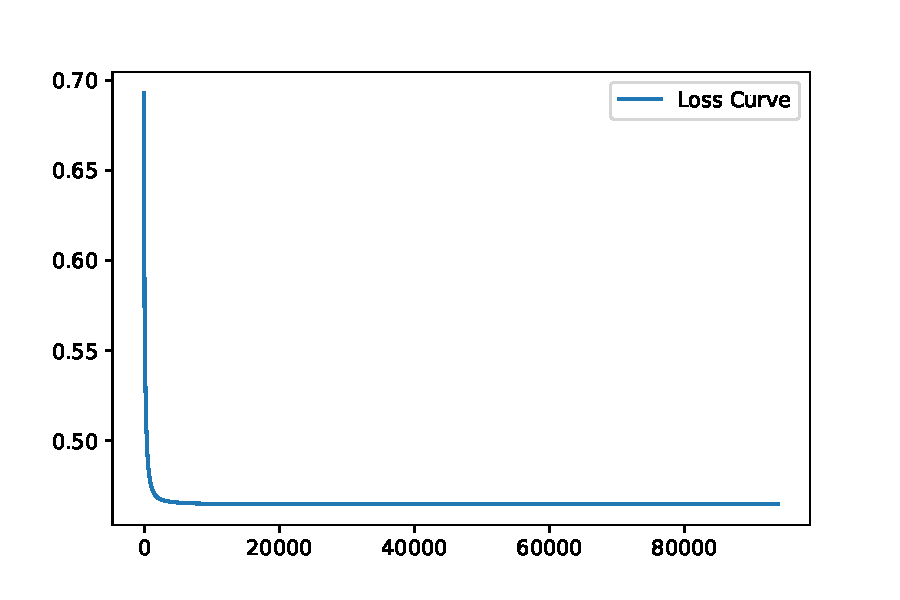
\includegraphics[width=6.5cm]{loss.pdf}
  \caption{total\_loss}
  \label{f5}
  \end{minipage}
\end{figure}
将训练过程中的准确率和累计损失的值绘图见图\ref{f4},\ref{f5},训练过程确实如之前我的直观感受。

对于预测测试结果如下:
\begin{itemize}
  \item Accuracy: 0.8882\\
  Test took: 0:01:07
\end{itemize}
准确率接近89\%.

\subsection{BERT与RNN模型对比分析}
上次LAB2的RNN模型的训练结果,256 隐藏单 RNN与256 隐藏2RNN当时的结果是:
\begin{quotation}
  Test Loss: 0.584 | Test Acc: 69.76\%

  Test Loss: 0.572 | Test Acc: 71.35\%
\end{quotation}

对比此次实验的BERT模型,在第一个epoch结束之后的数据已经是:
\begin{quotation}
  Average training loss: 0.33 | Accuracy: 88\%
\end{quotation}
训练损失值小于RNN但准确率远远高于RNN(由于训练的方式有一些区别因此损失值的结论可能不严谨,但准确率是RNN达不到的)。

但是,鉴于RNN是一个仅仅与输入层,隐藏层,输出层的网络,而BERT实际上是一个语言模型。语言模型通常采用大规模、
与特定NLP任务无关的文本语料进行训练,其目标是学习语言本身应该是什么样的的预训练模型。
BERT模型其预训练过程就是逐渐调整模型参数,使得模型输出的文本语义表示能够刻画语言的本质,便于后续针对具体NLP任务作微调。

因此显然对于训练imdb这个特定的语言数据集和,BERT拥有更好的训练结果。

% \bibliographystyle{gbt7714-numerical}
% % \bibliographystyle{7714-author-year}
% \bibliography{bibl}

\end{document}